\section{Impact of Thread Count}
Number of used threads plays a crucial role in execution duration of the code. We expect that as the number of threads go up the execution duration should decrease. We have executed the code for varying the parameter \texttt{NUMBER\_OF\_THREADS} from 1 to 5 for all different data and the plot the execution duration versus number of threads. 

\subsection{Birch3}
\begin{figure}[H]
\centering
\begin{tikzpicture}
\begin{axis}[
    xlabel={Number of Threads},
    ylabel={Execution Duration (seconds)},
    xmin=0.5, xmax=8.5,
    ymin=0..5, ymax=0.7,
    xtick={1, 2, 4, 6, 8},
    ytick={0.656673183, 0.337282581, 0.194313506, 0.123312713, 0.1061290290000 },
    ymajorgrids=true,
    grid style=dashed,
]
\addplot[
    color=orange,
    mark=*,
    ]
    coordinates {
    (1,0.656673183) (2,0.337282581) (4,0.194313506) (6,0.123312713) (8,0.106129029)
    };
\end{axis}
\end{tikzpicture}
\caption{Execution Duration vs. Number of Threads for Birch3}
\label{fig:birch}
\end{figure}

\subsection{Circle}
\begin{figure}[H]
\centering
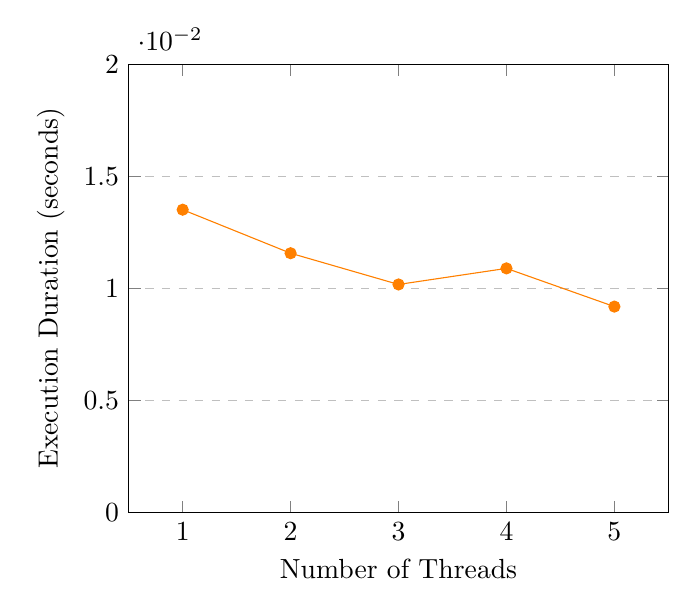
\begin{tikzpicture}
\begin{axis}[
    xlabel={Number of Threads},
    ylabel={Execution Duration (seconds)},
    xmin=0.5, xmax=5.5,
    ymin=0, ymax=0.02,
    xtick={1, 2, 3, 4, 5},
    ytick={0, 0.005, 0.01, 0.015, 0.02},
    ymajorgrids=true,
    grid style=dashed,
]
\addplot[
    color=orange,
    mark=*,
    ]
    coordinates {
    (1,0.013509184) (2,0.011566795) (3,0.010173890) (4,0.010891230) (5,0.009185814)
    };

\end{axis}
\end{tikzpicture}
\caption{Execution Duration vs. Number of Threads for Circle}
\label{fig:circle}
\end{figure}

\subsection{Hepta}
% Hepta
\begin{figure}[H]
\centering
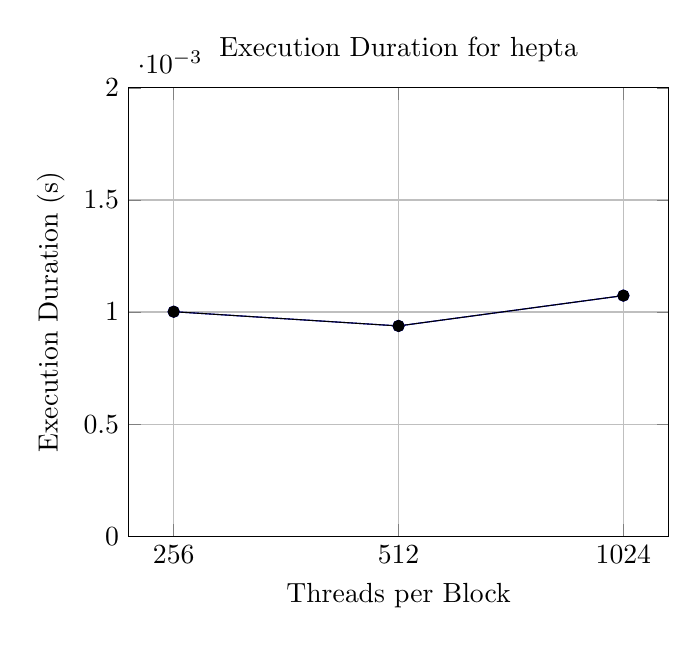
\begin{tikzpicture}
    \begin{axis}[
        xlabel={Threads per Block},
        ylabel={Execution Duration (s)},
        symbolic x coords={256, 512, 1024},
        xtick=data,
        ymin=0, ymax=0.002,
        grid=major,
        title={Execution Duration for hepta}
    ]
        \addplot coordinates {(256,0.00100147) (512,0.000937984) (1024,0.00107334)};
        \addplot[mark=*] coordinates {(256,0.00100147) (512,0.000937984) (1024,0.00107334)};
    \end{axis}
\end{tikzpicture}
\caption{Comparison of execution duration for the dataset Hepta: N212 with different
threads per thread block. Experiments are conducted on an NVIDIA RTX4070 consumer GPU}
\end{figure}

\subsection{Isolation}
\begin{figure}[H]
\centering
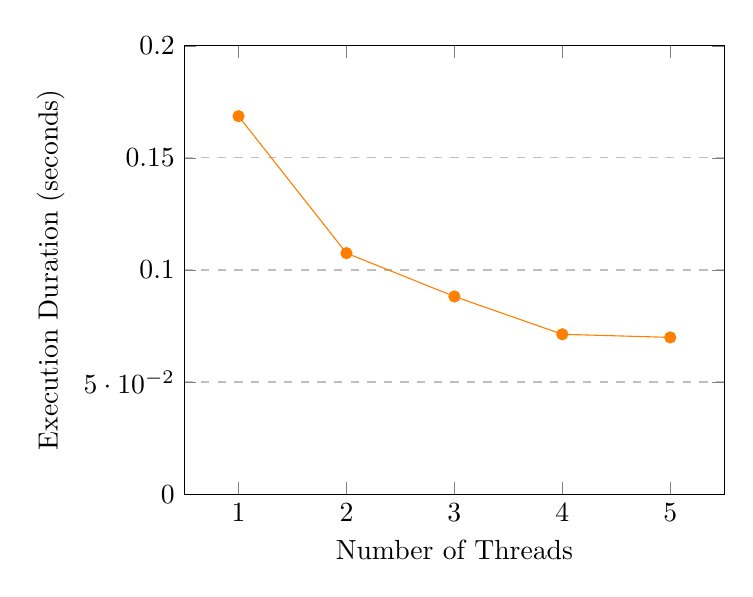
\begin{tikzpicture}
\begin{axis}[
    xlabel={Number of Threads},
    ylabel={Execution Duration (seconds)},
    xmin=0.5, xmax=5.5,
    ymin=0, ymax=0.2,
    xtick={1, 2, 3, 4, 5},
    ytick={0, 0.05, 0.1, 0.15, 0.2},
    ymajorgrids=true,
    grid style=dashed,
]

\addplot[
    color=orange,
    mark=*,
    ]
    coordinates {
    (1,0.168613077) (2,0.107514931) (3,0.088181996) (4,0.071310858) (5,0.069919249)
    };

\end{axis}
\end{tikzpicture}
\caption{Execution Duration vs. Number of Threads for Isolation}
\label{fig:isolation}
\end{figure}

\subsection{Smile}
\begin{figure}[H]
\centering
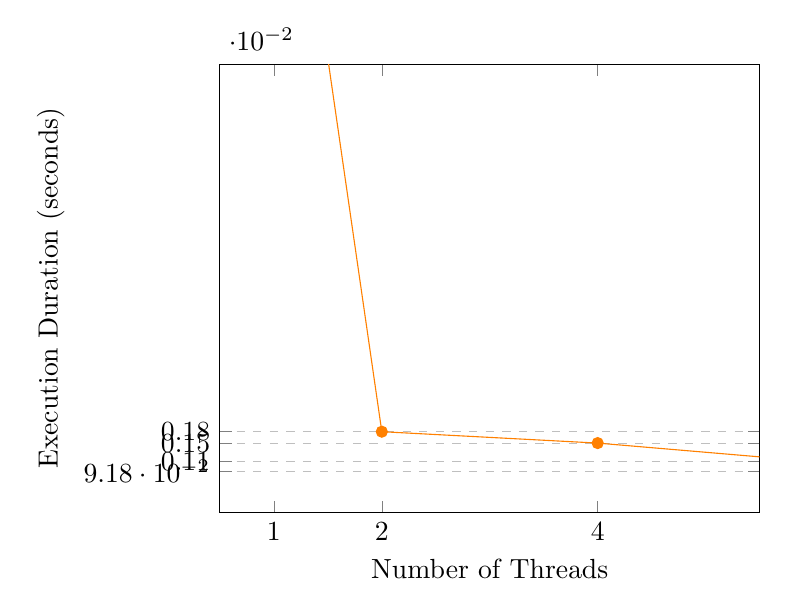
\begin{tikzpicture}
\begin{axis}[
    xlabel={Number of Threads},
    ylabel={Execution Duration (seconds)},
    xmin=0.5, xmax=5.5,
    ymin=0, ymax=0.01,
    xtick={1, 2, 4, 6, 8},
    ytick={0.018443924, 0.00180292, 0.001548536, 0.00113928, 0.000918407},
    ymajorgrids=true,
    grid style=dashed,
]

\addplot[
    color=orange,
    mark=*,
    ]
    coordinates {
    (1,0.018443924) (2,0.00180292) (4,0.001548536) (6,0.001139281) (8,0.000918407)
    };

\end{axis}
\end{tikzpicture}
\caption{Execution Duration vs. Number of Threads for Smile}
\label{fig:smile}
\end{figure}


We can see that there is not an absolute monotonic decaying behavior observed when the thread number increased. This might occur in data such that the number of data-points are small and the atomic operations make the execution more time consuming. This behavior can be observed in the figures \ref{fig:circle}, \ref{fig:hepta} and \ref{fig:smile}. It can be observed from the figure \ref{fig:birch} when the data points are relatively large, increasing the thread number results in a monotonic decaying execution duration. 

